\documentclass{article}
\usepackage{graphicx} % Required for inserting images
\usepackage{float}
\title{VDL1}
\author{Erik Schwede}
\date{November 2023}

\begin{document}

\maketitle

\section{}
\subsection{}
\subsection{}
\subsubsection{}
Due to the chain rule that is used in the back propargation. Every derivitive is multiplied by each other. If there are some realy smal values, the overall derivitive is also going to be close to 0. Wich will limit the learning effect of the neural network.
\subsubsection{}
$\sigma(x) = \frac{1}{1 + e^{-x}}$\\\\
$\sigma'(x) = \frac{e^x}{(e^{x} + 1)^2}$\\\\
$\sigma''(x) = \frac{(e^x-1)e^x}{(e^{x} + 1)^3}$\\\\
$\sigma''(x) = 0$\\\\
$0 = e^x$\\\\
$\lim \limits_{x \to -\infty} e^x = 0$\\\\
$\lim \limits_{x \to -\infty} \sigma'(x) = 0$\\\\
$0 = e^x-1$\\\\
$1 = e^x$\\\\
$x = 0$\\\\
$\sigma'(0) = \frac{e^0}{(e^{0} + 1)^2} = 0.25$\\
\begin{figure}[H]
    \centering
    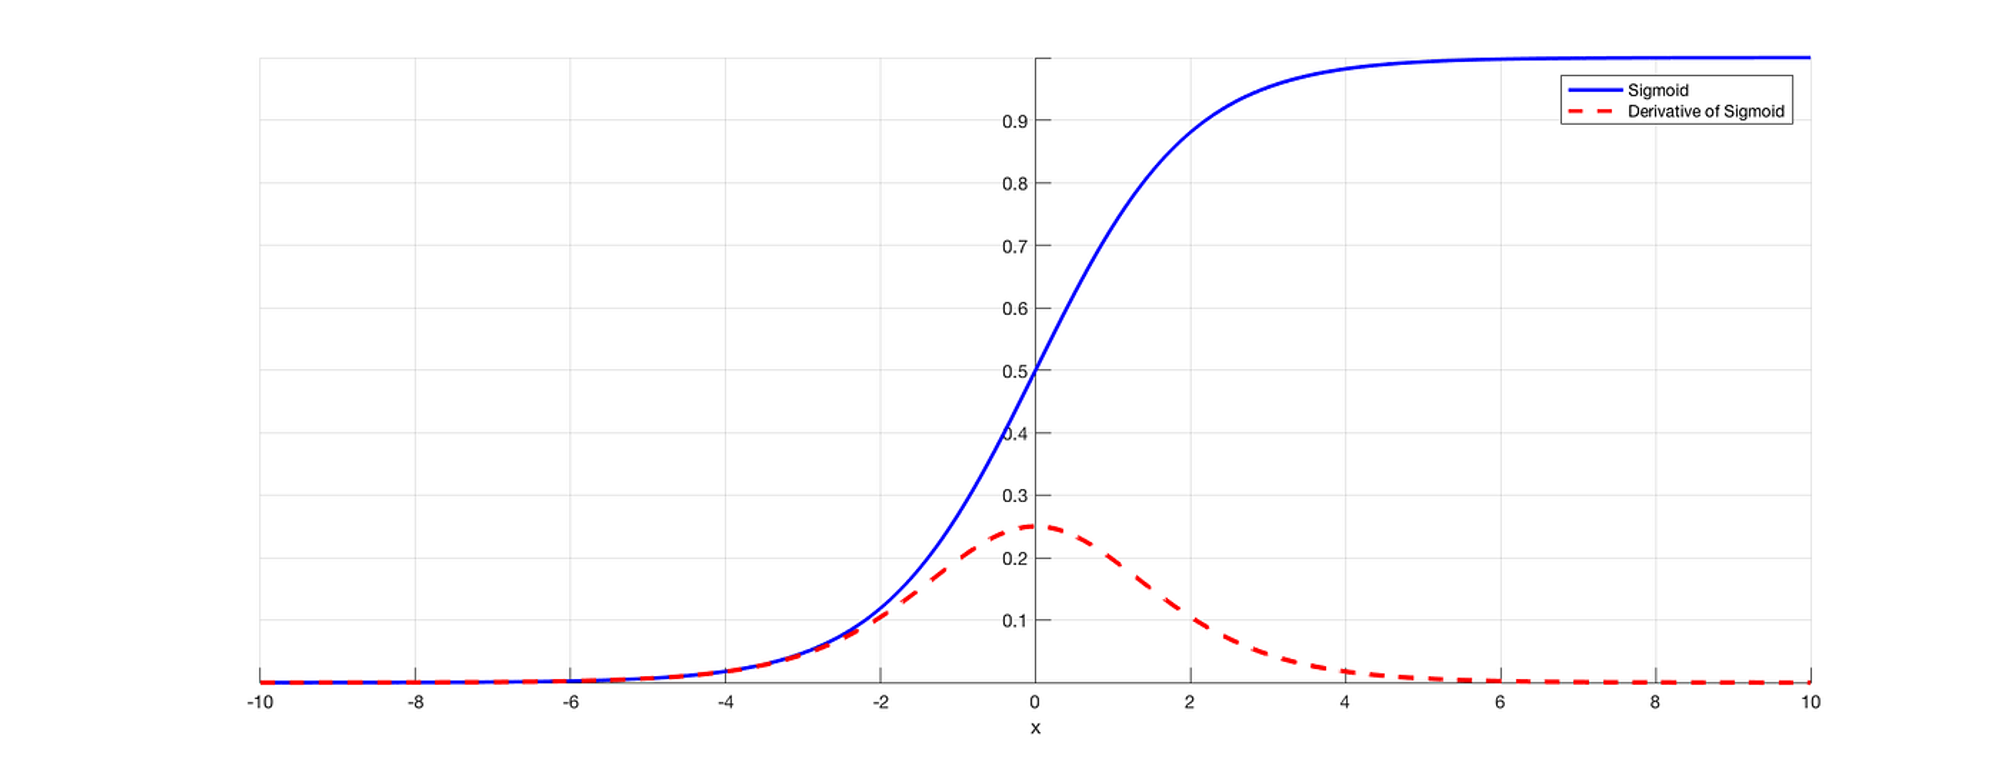
\includegraphics[width=\textwidth]{sigmoid.png}
    \caption{$\sigma(x)$ and $\sigma'(x)$ functions}
\end{figure}

According to these calculations the upperbound of the derivitive of the sigmoid function is $0.25$ and the lowerbound is close to $0$ but never reaches $0$ due to the caracteristics of the $e$-function.
\subsubsection{}
$a_{1} = \sigma(w_{1}x)$\\
$a_{2} = \sigma(w_{2}a_{1})$\\
$a_{3} = \sigma(w_{3}a_{2})$\\
$a_{4} = \sigma(w_{4}a_{3})$\\
$y = \sigma(w_{5}a_{4})$\\\\
$\frac{\partial y}{\partial x} = \frac{\partial y}{\partial a_{4}} \cdot \frac{\partial a_{4}}{\partial a_{3}} \cdot \frac{\partial a_{3}}{\partial a_{2}} \cdot \frac{\partial a_{2}}{\partial a_{1}} \cdot \frac{\partial a_{1}}{\partial x} = w_{5}\sigma'(a_{4}) \cdot w_{4}\sigma'(a_{3}) \cdot w_{3}\sigma'(a_{2}) \cdot w_{2}\sigma'(a_{1}) \cdot w_{1}\sigma'(x)$\\\\
$\frac{\partial y}{\partial x} = w_{5}w_{4}w_{3}w_{2}w_{1} \cdot \sigma'(x)\sigma'(a_{1})\sigma'(a_{2})\sigma'(a_{3})\sigma'(a_{4})$
\subsubsection{}
In the context of the sigmoid function, its derivative $\sigma'$ has an upper bound of $0.25$. When this derivative is used in the chain rule during back propagation, it is multiplied with the weights for each layer. If the weights are less than $1$, the gradients will diminish as they are back propagated through the layers. This means that the farther back you go in the network, the smaller the gradients become, potentially approaching zero. As a result, the weights in the early layers receive very small updates, and these layers may not learn effectively during training.
\subsubsection{}
Exploding gradients refer to a situation in deep learning where the gradients during back propagation become extremely large. This can lead to numerical instability and cause the weights of the neural network to update excessively, potentially resulting in the model's failure to converge during training. 
Exploding gradient problem in sigmoid activation can happen when the initial weights of the network are very large along with large number of layers. This would happen because sigmoid transform an input space into a space that is between [0,1]. So for large input values the gradients could collect during an update, resulting in very big gradients, which eventually results in huge modifications to network weights, resulting in an unstable network and causing exploding gradients problem.

\end{document}
